\subsection{Cinemática diferencial}
\subsubsection{Jacobiano lineal por derivación}
El procedimiento de clase toma la posición de $M_{03}$ y deriva cada componente respecto de las variables articulares \parencite{course6,course7}:
\begin{equation}
\dot P_{03}=J_L(q)\dot q,\qquad
(J_L)_{ij}=\frac{\partial (P_{03})_i}{\partial\theta_j}.
\end{equation}
Por ejemplo, $\partial p_x/\partial\theta_1=-s_1\rho$, $\partial\rho/\partial\theta_2=-z_r$ y $\partial\rho/\partial\theta_3=-l_3s_{23}$. Por tanto,
\begin{equation}
J_L=\begin{bmatrix}
-s_1\rho&-c_1z_r&-l_3c_1s_{23}\\
c_1\rho&-s_1z_r&-l_3s_1s_{23}\\
0&\rho&l_3c_{23}
\end{bmatrix}.
\end{equation}
Las unidades de sus entradas son m/rad. El desplazamiento fijo $l_1$ desaparece al derivar. En el código, $J_L$ corresponde a la primera matriz devuelta por \texttt{jacobian}; la denominación anterior $J_v$ representa la misma matriz.

\subsubsection{Jacobiano angular y comprobación geométrica}
Para las tres articulaciones rotacionales, la semana 7 construye $J_\omega=[z_0\ z_1\ z_2]$, con ejes expresados en la base. En este modelo:
\begin{equation}
z_0=\begin{bmatrix}0\\0\\1\end{bmatrix},\quad
z_1=z_2=\begin{bmatrix}s_1\\-c_1\\0\end{bmatrix},\quad
J_\omega=\begin{bmatrix}0&s_1&s_1\\0&-c_1&-c_1\\1&0&0\end{bmatrix}.
\end{equation}
Así,
\begin{equation}
\begin{bmatrix}v\\\omega\end{bmatrix}
=\underbrace{\begin{bmatrix}J_L\\J_\omega\end{bmatrix}}_{J\in\mathbb R^{6\times3}}\dot q.
\end{equation}
Cada columna lineal también se obtiene de $z_{i-1}\times(P_{03}-o_{i-1})$. Las pruebas comparan ambas construcciones y verifican la parte angular mediante $[\omega]_\times=\dot R R^T$. Esta velocidad angular no equivale, en general, a derivar tres ángulos de Euler: esa parametrización utiliza un Jacobiano analítico diferente.

\subsubsection{Comprobación de velocidades}
Una trayectoria articular suave prescribe $q(t)$ y $\dot q(t)$. Se contrasta $J_L\dot q$ con la diferencia central $[P(t+\Delta t)-P(t-\Delta t)]/(2\Delta t)$. Para $\Delta t=0.01$ s, el error máximo es aproximadamente $3.99\times10^{-7}$ m/s. Al dividir el paso por dos, el error se reduce aproximadamente por cuatro, consistente con la diferencia central. Se excluyen los extremos del intervalo.
\begin{figure}[htbp]\centering
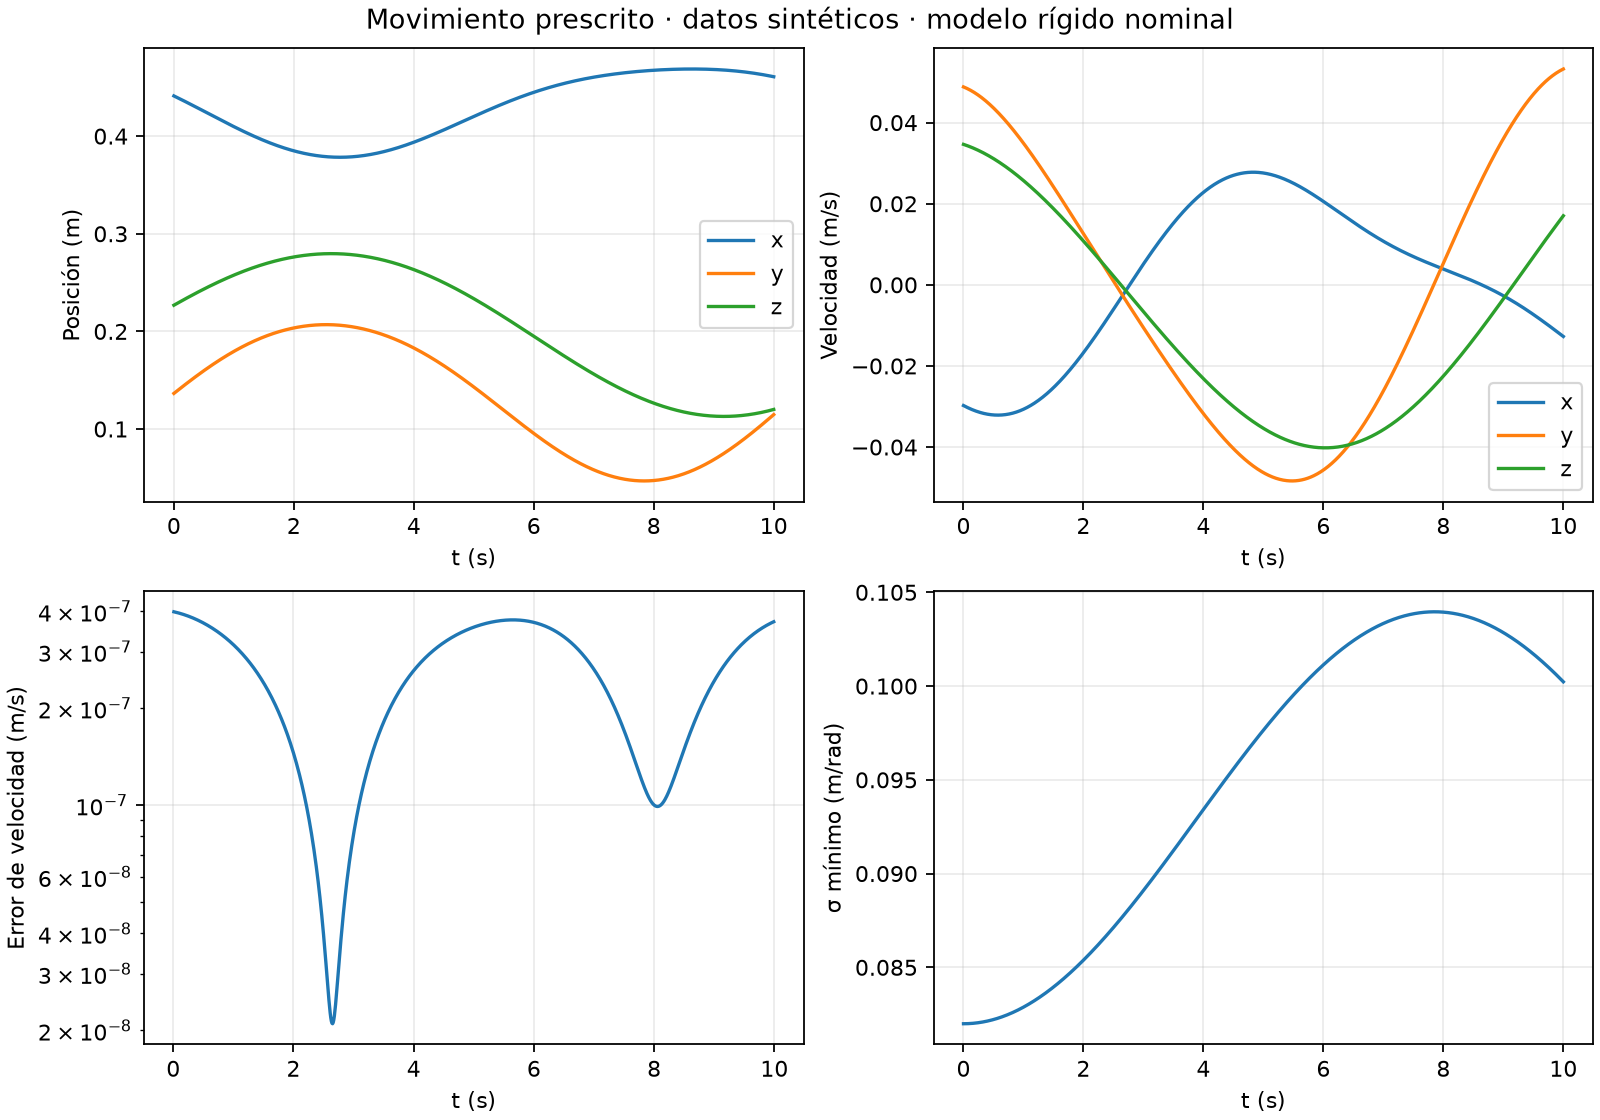
\includegraphics[width=.90\linewidth]{../simulations/differential/results/run-001/diagnostics.png}
\caption{Comprobación del Jacobiano lineal sobre movimiento prescrito. No corresponde a control en lazo cerrado.}
\end{figure}
